\section{Estimation of the angular measure\label{sec:methodology}}

Our approach to estimating the PoT distribution considers two steps: First we 
    estimate the shape and scale parameters for the
    multivariate Pareto distribution, using the univariate marginals; Then 
    we focus on the dependence structure in extreme regions by proposing a 
    flexible model for the distribution of $\bm{V}$. Consider a collection of 
    observations  $\bm{w}_i \in {\mathbb R}^d, i = 1, \ldots, n$ that exhibit 
    extreme behavior.  We start by setting a large threshold 
    $b_{t,\ell}$ for the  $\ell$-th marginal, $\ell = 1, \ldots,d$. Then, the 
    distribution of the observations for the $\ell$-th component, 
    conditional on exceeding the threshold, can be 
    approximated as $1 - (1 + \xi_\ell   (w_{i\ell} - b_{t,\ell})/\sigma_\ell)_+^
    {1/\xi_ell}$, where $(\cdot)_+$ indicates the positive part function.  We 
    proceed by setting a threshold equal to the empirical $(1-1/t)$-quantile. 
    Thus $b_{t,l}  = \hat{F}^{-1}_{\ell}(1 - 1/t)$.  We then use the 
    approximate exceedance distribution to estimate $\xi_\ell$ and $\sigma_\ell$,
    for each $\ell$, using likelihood based methods. Then, in order to estimate 
    the angular distribution, we use those estimates to standardize each of 
    the marginals. The standardization yields
    \begin{equation}
            \label{eqn:standardization}
            z_{i\ell} = \left(1 + \xi_{\ell}\frac{w_{i\ell} -
                b_{\ell}}{a_{\ell}}\right)_{+}^{1/\xi_{\ell}}\; .
        \end{equation}
    Note that $z_{i\ell}> 1$ implies that $w_{i\ell} > b_{t,\ell}$, meaning 
    that the observation $\bm{w}_i$ is extreme in the $\ell$-th dimension. 
    Thus, $r_i = \|\bm{z}_i\|_\infty > 1$ implies that at
    least one dimension has an extreme observation, and corresponds 
    to a very extreme observation when $t$ is large. We focus on 
    the observations that are such that $r_i > 1$. These provide a
    sub-sample of $r_i$ and $\bm{v}_i = \bm{z}_i /r_i \in 
    \mathbb{S}_{\infty}^{d-1}$ that is used for  the estimation of 
    $\Phi$ conditional on the sample. We observe that in practice, the choice
    of $\bm{b}$, and the subsequent fitting of $\bm{a}$ and $\bm{\xi}$ induces
    a stochastic element in the spectral distribution that is not accounted for
    in our analysis.  \makenote{phrasing?}

\subsection{Projected gamma family\label{subsec:projgamma}}
To obtain a distribution on 
${\mathbb S}_{p}^{d-1}=\{\bm{s} : \bm{s} \in {\mathbb R}_{+}^{d}, \| \bm{s}\|_{p} = 1\}$ 
we start with a vector in 
$\bm{x} \in {\mathbb R}^d_+$, calculate its $\mathcal{L}_p$-norm  defined as
  \begin{equation*}
    \lVert \bm{x} \rVert_p = 
    \left({\textstyle\sum}_{\ell = 1}^d \lvert s_{\ell}\rvert^p\right)^{\frac{1}{p}},
  \end{equation*}
  and normalize it to obtain $\bm{y} = \bm{x}/\|\bm{x}\|_p \in {\mathbb S}_p^{d-1}$. 
  The absolute and Euclidean norms are obtained for $p=1$ and $p=2$ respectively,
  and the $\mathcal{L}_{\infty}$ norm can be obtained as a limit, 
  \begin{equation*}
    \| \bm{s} \|_{\infty}
      = \lim\limits_{p\to\infty} \| \bm{s} \|
      = \underset{\ell = 1}{\overset{d}{\bigvee}}s_{\ell}.
  \end{equation*}

A natural  distribution to consider in ${\mathbb R}^d_+$ is given by a product of independent
  univariate Gamma distributions. Let
    $\bm{ X} \sim \prod_{\ell = 1}^d\text{Ga}\left(X_{\ell}\mid\alpha_{\ell},\beta_{\ell}\right)$, 
    $\alpha_\ell$ and $\beta_\ell$ are the shape and scale parameters, respectively. 
    For any finite $p$, letting 
   $ y_d = (1 - {\textstyle\sum}_{\ell = 1}^{d-1}y_{\ell}^p)^{1/p}$,
    the transformation
  \begin{equation}
    \label{eqn:pnormt}
    \begin{aligned}
    T(x_1,\ldots,x_d) &= \left(\pnorm{\bm{x}}{p}, \frac{x_1}{\pnorm{\bm{x}}{p}},
                          \ldots , \frac{x_{d-1}}{\pnorm{\bm{x}}{p}}\right) \\
                        &= (r,y_1,\ldots,y_{d-1})
    \end{aligned}
  \end{equation}
  is invertible with
  \begin{equation}
    \label{eqn:pnormtinv}
    \begin{aligned}
    &\hspace{-0.5cm}T^{-1}\left(r,y_1,\ldots,y_{d-1}\right)\\
      & = \left(ry_1,\ldots,ry_{d-1}, 
        r\left(1 - {\textstyle\sum}_{\ell = 1}^{d-1}y_{\ell}^p\right)^{\frac{1}{p}}\right).
    \end{aligned}
  \end{equation}
  The Jacobian of the transformation takes the form
  \begin{equation}
    \label{eqn:pnormjac}
    \begin{aligned}
    r^{d-1}\left[\left(1 - {\textstyle\sum}_{\ell = 1}^{d-1}y_{\ell}^p\right)^{\frac{1}{p}} \right. & \\
        &\hspace{-2cm}+ \left. {\textstyle\sum}_{\ell = 1}^{d-1}y_{\ell}^p
          \left(1 - {\textstyle\sum}_{l=1}^{d-1} y_{\ell}^p\right)^{\frac{1}{p} - 1}\right].
    \end{aligned}
  \end{equation}
  The normalization provided by $T$ maps a vector in ${\mathbb R}_+^d$ onto
  ${\mathbb S}_p^{d-1} $. With a slight abuse of terminology we refer to it as a
  projection. Using Equations (\ref{eqn:pnormt}) -- (\ref{eqn:pnormjac}) we have the joint density
  \begin{equation}
  \label{joint}
    \begin{aligned}
    f(r,\bm{ y}) = &\prod_{\ell = 1}^{d}
      \left[\frac{\beta_{\ell}^{\alpha_{\ell}}}{\Gamma(\alpha_{\ell})}(ry_{\ell})^{\alpha_{\ell} - 1}
          \exp\lbrace-\beta_{\ell}ry_{\ell}\rbrace\right] \\
      &\hspace{0.5cm}\times r^{d-1}\left[y_d +
            {\textstyle \sum}_{\ell = 1}^{d-1}y_{\ell}^p\left(y_d^p\right)^{\frac{1}{p} - 1}\right].
    \end{aligned}
  \end{equation}
  Integrating out $r$ yields the resulting \emph{Projected Gamma} density
  \begin{equation}
    \label{eqn:projgamma}
    \begin{aligned}
    \text{PG}(\bm{ y}\mid\bm{ \alpha},\bm{ \beta}) &=
          \prod_{\ell = 1}^d\left[\frac{\beta_{\ell}^{\alpha_{\ell}}}{\Gamma(\alpha_{\ell})}
                y_{\ell}^{\alpha_{\ell} - 1}\right]\\
      &\hspace{0.5cm}\times \left[y_d +
          {\textstyle \sum}_{\ell = 1}^{d-1}y_{\ell}^p\left(y_d^p\right)^{\frac{1}{p} - 1}\right]\\
      &\hspace{0.5cm}\times \frac{\Gamma({\textstyle\sum}_{\ell = 1}^d\alpha_{\ell})}{\left({\textstyle\sum}_{\ell = 1}^d
                    \beta_{\ell}y_{\ell}\right)^{{\scriptstyle\sum_{\ell = 1}^d \alpha_{\ell}}}},
    \end{aligned}
  \end{equation}
  defined for $\bm{y}\in {\mathbb S}_p^{d-1}$, and for any finite $p>0$. To avoid identifiability 
  problems when estimating the shape and scale parameters, we set $\beta_1 = 1$.
  \cite{nunez2019} obtain the density in Equation (\ref{eqn:projgamma})
  for $p=2$ as a multivariate distribution for directional data, using spherical coordinates.  
  For $\bm{ y}\in {\mathbb S}_1^{d-1}$, and $\beta_{\ell} = \beta$ for all $\ell$, the density in Equation (\ref{eqn:projgamma}) corresponds to that of a Dirichlet distribution.
  
  
The projected gamma family is simple to specify and has very tractable 
  computational properties. Thus, we use it as a building block for the 
  angular measure $\Phi$ models. To build a flexible family of distributions 
  in ${\mathbb S}_p^{d-1}$ we consider mixtures of projected gamma densities 
  defined as
  \begin{equation} \label{eqn:PGmix}     
     f(\bm{y}) = \int_\Theta \mathcal{PG}(\bm{y}\mid \bm{\theta}) dG(\bm{\theta}), 
  \end{equation} 
where $\bm{\theta} = (\bm{\alpha}, \bm{\beta})$. Following a Bayesian 
  non-parametric approach \citep{Ferguson74,Antoniak1974} we assume that $G$ 
  is drawn from a random measure. In particular, assuming a Dirichlet process 
  prior for $G$, we have a hierarchical formulation of the mixture model that, 
  for a vector of observations $\bm{y}_i$, is given by
  \begin{equation}\label{eqn:dppg}
    \begin{aligned}
    \bm{y}_i &\sim \text{PG}(\bm{y}_i\mid \bm{\theta}_i)\\
    \bm{\theta}_i &\sim G
    \end{aligned}
    ~\hspace{1cm}
    \begin{aligned}
    G &\sim \mathcal{DP}(\eta, G_0),
    \end{aligned}
  \end{equation}
  where $\mathcal{DP}$ denotes a Dirichlet process, $\eta$ is the precision 
  parameter, and $G_0$ is the centering distribution. 
  
Unfortunately, in the limit when $p\rightarrow \infty$, the projection 
  transformation is not differentiable. Thus, a closed form expression 
  like Equation (\ref{eqn:projgamma}) for the projected gamma density on ${\mathbb S}_\infty^{d-1}$ is not 
  available. Instead, we observe that for a sufficiently large $p$, $\mathbb{S}_p^{d-1}$ will approach
  $\mathbb{S}_{\infty}^{d-1}$.  With that in mind, our strategy consists of describing the angular
  distribution $\Phi$ using a sample based approach with the following steps: (i) Apply the 
  transformation in Equation (\ref{eqn:standardization}) to the original data; (ii) Obtain the 
  subsample of the standardized observations that satisfy $R>1$; (iii) Take a finite $p$ and 
  project the observations onto ${\mathbb S}_p^{d-1}$; 
  (iv) Fit the model in Equation (\ref{eqn:PGmix}) to the resulting 
  data and obtain samples from the fitted model; 
  (v) Project the resulting samples onto ${\mathbb S}_\infty^{d-1}$.
  For step (iv) we use a Bayesian approach that is implemented using a purposely 
  developed Markov chain Monte Carlo sampler described in the next section.

\begin{figure}[ht]
    \centering
    \caption{The positive orthant of the $p$-norm sphere.}
  \begin{subfigure}[b]{0.4\textwidth}
    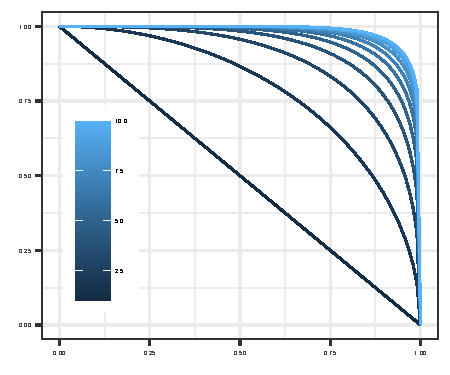
\includegraphics[width=\textwidth]{./images/p_sphere}
    \caption{${\mathbb S}_p^1$ for $p = 1,\ldots, 10$\label{fig:psphere}}
  \end{subfigure}
  %
  \begin{subfigure}[b]{0.4\textwidth}
    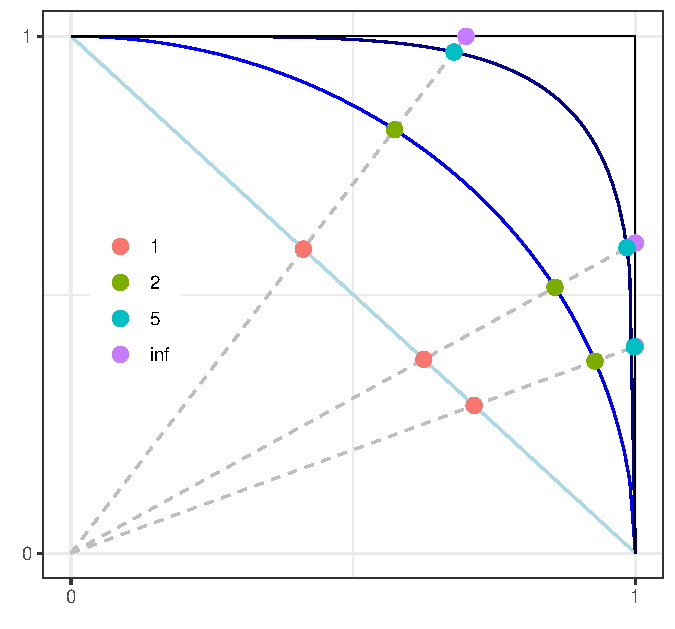
\includegraphics[width=\textwidth]{./images/p_project}
    \caption{Projection of data on ${\mathbb S}_{\infty}^1$ onto ${\mathbb S}_p^1$\label{fig:pproject}}
  \end{subfigure}
\end{figure}

A measure that is used to characterize the strength of the dependence,
  in the tail, for two random variables $Z_1$ and $Z_2$, with marginal
  distributions $F_1$ and $F_2$ is given by \citep{coles2001}
  \[
    \chi_{12} = \lim\limits_{u\uparrow 1} \prob{F_1(Z_1)>u\mid F_2(Z_2)>u}.   
  \]
  $\chi_{12}$ provides information about the distribution of extremes for the variable $Z_1$
  given that $Z_2$ is very large.  When $\chi_{12}>0$, $Z_1$ and $Z_2$ are said to
  be asymptotically dependent, otherwise they are asymptotically independent. The following result 
  provides the asymptotic dependence coefficient between two components of $\bm{Z}$ after PoT limit.
  \begin{prop}\label{ppchi}
  Suppose that $\bm{Z} = R\bm{V}$ with $R\sim Pa(1)$,
  $\prob{V_\ell > 0} = 1$ and $\expect{V_\ell}$ exists, for $\ell=1, \ldots ,d$, then
    \begin{equation}
    \label{eqn:chi_ij}
	\chi_{\jmath\ell} = \expect{\frac{V_\jmath}{\expect{V_\jmath}} \wedge \frac{V_\ell}{\expect{V_\ell}}}
    \end{equation}
  \end{prop}
  {\em Proof:}
  Denote as $F_\ell$ the marginal distribution of $Z_\ell$. To obtain $\chi_{\jmath\ell}$ we need 
  $Pr(Z_\jmath>z_\jmath,Z_\ell>z_\ell)$, where $z_\ell = F_\ell^{-1}(u) = \expect{V_\ell}/(1 - u), \;\ell=1,\dots, d$.  
  Using the fact that $V_\ell>0, \forall \ell$ almost surely, we have that the former is equal to
  \begin{equation*}
    \begin{aligned}
    &\hspace{-0.5cm}\prob{R>\frac{z_\jmath}{V_\jmath}\vee\frac{z_\ell}{V_\ell}}
    = \expect{1\wedge\left(\frac{z_\jmath}{V_\jmath}\vee\frac{z_\ell}{V_\ell}\right)^{-1}}\\
    &= \expect{\frac{V_\jmath}{z_\jmath}\wedge\frac{V_\ell}{z_\ell}}
    = (1 - u)\expect{\frac{V_\jmath}{\expect{V_\jmath}}\wedge\frac{V_\ell}{\expect{V_\ell}}},
    \end{aligned}
  \end{equation*}
  where the second identity is justified by the fact that $V_i$ is bounded and $z_i\rightarrow\infty$. The 
  proof is completed by noting that $\prob{F_i(Z_i)>u} = 1 - u. \hfill\Box$

Equation \ref{eqn:chi_ij} implies that $\chi_{\jmath\ell}>0$, and so, no asymptotic independence is possible 
  under our proposed model. For the analysis of extreme values it is of interest to calculate the multivariate 
  conditional survival function. The following result provides the relevant expression, as a function of the 
  angular measure.
  \begin{prop}
  Assume the same conditions of Proposition \ref{ppchi}.   Let $\alpha \subset \{1, \ldots ,d\}$ be a 
  collections of indexes.  Then     
  \begin{equation} \label{eqn:condsurv}
    \begin{aligned}
    &\hspace{-0.5cm}\mathrm{Pr}\left[\bigcap_{\ell \in \alpha} 
        Z_\ell > z_\ell \mid \bigcap_{\ell\not\in\alpha} Z_\ell > z_\ell\right] \\
    &= \frac{\expect{\bigwedge_{k = 1}^d 1\wedge \frac{V_k}{z_k}}}{\expect{\bigwedge_{k \not\in\alpha}1\wedge\frac{V_k}{z_k}}}.
    \end{aligned}
  \end{equation}
  \end{prop}  
  The proof uses a similar approach to the proof of Proposition \ref{ppchi}.

Equations \ref{eqn:chi_ij} and \ref{eqn:condsurv} provide relevant tools for inference on the tail 
  behavior of the joint distribution of the observations. The expressions can be readily calculated 
  within a sample-based inferential approach like the one considered in the following section.


\subsubsection{Inference for the projected Gamma mixture model}
In a sample-based inference approach, for a given iteration the Dirichlet process mixture model groups observations
    into stochastically assigned clusters, where members of a cluster share distributional parameters. Building out 
    the methods of inference for Equation~(\ref{eqn:dppg}), 
    let $n_j^{-i}$ be the number of observations in cluster $j$ not including observation $i$.  Let $J^{-i}$ be 
    the number of extant clusters, not including any singleton that observation $i$ is in. Under this model, 
    the probability of cluster membership for a given observation is proportional to
\begin{equation*}
    \text{Pr}\left[\delta_i = j\mid\ldots\right] \propto \begin{cases}
        n_j^{-i}\mathcal{PG}\left(\bm{y}_i\mid\bm{\alpha}_j,\bm{\beta}_j\right)\\ % \hspace{0.5cm} \\ % &\text{~for~}j \in \lbrace 1,\ldots,J^{-i}\rbrace\\
        \eta\int\mathcal{PG}\left(\bm{y}_i\mid\bm{\alpha}_j,\bm{\beta}_j\right)dG_0(\bm{\alpha}_j,\bm{\beta}_j),%\hspace{0.5cm} % &\text{~for~}j = J^{-i} + 1.
        \end{cases}
\end{equation*}
where the top case is iterating over extant clusters $j = 1,\ldots, J^{-i}$, and the bottom case is
    for a \emph{new} cluster. If $G_0$ is not a conjugate prior for the kernel density, the integral in the 
    above formula may not be available in closed form. We sidestep this using Algorithm 8 from \cite{neal2000}: 
    by Monte Carlo integration, we draw $m$ candidate clusters, $\bm{\alpha}_j,\bm{\beta}_j$ for
    $j = J^{-i} + 1,\ldots, J^{-i} + m$ from $G_0$. Then, we sample the cluster indicator 
    $\gamma_i$ from extant or candidate clusters, where the probability of cluster membership is proportional to
\begin{equation}
    \text{Pr}\left[\delta_i = j\mid\ldots\right] \propto \begin{cases}
        n_j^{-i}\mathcal{PG}\left(\bm{y}_i\mid\bm{\alpha}_j,\bm{\beta}_j\right)\\ % \hspace{0.5cm}  % &\text{~for~}j \in \lbrace 1,\ldots,J^{-i}\rbrace\\
        \frac{\eta}{m}\mathcal{PG}\left(\bm{y}_i\mid\bm{\alpha}_j,\bm{\beta}_j\right). % \hspace{0.5cm} &\text{~for~}j \in \lbrace J^{-i} + 1,\ldots, J^{-i} + m\rbrace.
        \end{cases}
\end{equation}
Again, the top case is iterating over extant clusters, and now the bottom case is iterating 
    over new \emph{candidate} clusters.  If a candidate cluster is selected,
%{\bf you first have to say that you sample from this distribution. What is the ``candidate cluster''?}
    then $\gamma_i = J = J^{- i} + 1$, and the associated cluster parameters are saved.

A key feature of the the projected Gamma distribution is its computational properties. We augment 
$\mathcal{PG}(\bm{y}_i\mid\bm{\alpha}_i,\bm{\beta}_i) $ by introducing a latent radial component $r_i$, 
for each observation. Using Equation \eqref{joint} we observe that the 
full conditional of $r_i$ is easy to sample from, as it is given as
\begin{equation}
    r_i\mid\bm{\alpha}_i,\bm{\beta}_i \sim \mathcal{G}\left(r_i \bigmid \sum_{\ell = 1}^d\alpha_{i\ell}, \sum_{\ell = 1}^d\beta_{\ell} y_{i\ell}\right).
\end{equation}
Moreover,  the full conditional for $\bm{\alpha}_j,\bm{\beta}_j$ is then proportional to
\begin{equation}
    \begin{aligned}
    &\hspace{-1cm}f(\bm{\alpha}_j,\bm{\beta}_j\mid \bm{Y},\bm{r},\bm{\delta},\ldots) \\
    &\propto \prod_{i:\gamma_i = j}\prod_{\ell = 1}^d\mathcal{G}\left(r_iy_{i\ell}\mid\alpha_{j\ell},\beta_{j\ell}\right) \\
    &\hspace{0.5cm} \times dG_0(\bm{\alpha}_j,\bm{\beta}_j).
    \end{aligned}
\end{equation}
Note that the ordering of the products can be reversed in the likelihood, indicating that given $\bm{r}$, 
the likelihood becomes separable by dimension.
We first consider a centering distribution given by a product of independent Gammas:
\begin{equation}
    \begin{aligned}
    &\hspace{-0.3cm}G_0(\bm{\alpha}_j,\bm{\beta}_j\mid \bm{\xi},\bm{\tau},\bm{\zeta},\bm{\sigma}) \\
    &= \prod_{\ell = 1}^d\mathcal{G}(\alpha_{j\ell}\mid \xi_{\ell},\tau_{\ell})\times\prod_{\ell = 2}^d\mathcal{G}(\beta_{j\ell}\mid\zeta_{\ell},\sigma_{\ell}).
    \end{aligned}
\end{equation}
This model is completed with independent Gamma priors on $\xi_{\ell}$, $\tau_{\ell}$, $\zeta_{\ell}$, $\sigma_{\ell}$.  We also assume a Gamma prior on $\eta$, that is updated via the procedure outlined in \cite{escobar1995}.  We refer to this model as the \emph{projected Gamma--Gamma} (PG--G) model.  An advantage of the PG--G model is that, thanks to conjugacy, the rate parameters can easily be integrated out for inference on $\bm{\alpha}_j$.  Then, the full conditional for $\alpha_{j\ell}$ takes the form
\begin{equation}
    \label{eqn:alphalupdate}
    \begin{aligned}
    &\hspace{-0.5cm}\pi(\alpha_{j\ell}\mid \bm{r},\bm{Y},\bm{\gamma},\xi_\ell,\tau_\ell,\zeta_\ell,\sigma_\ell) \\
    &\propto \frac{\left(\prod_{i:\gamma_i = j}r_iy_{i\ell}\right)^{\alpha_{j\ell} - 1}\alpha_{j\ell}^{\xi_\ell - 1}e^{-\tau_\ell \alpha_{j\ell}}\times}{\Gamma^{n_j}(\alpha_{j\ell})} \\
    &\hspace{0.5cm}\times \frac{\Gamma\left(n_j\alpha_{j\ell} + \zeta_{\ell}\right)}{\left(\sum_{i:\gamma_i = j}r_iy_{i\ell} + \sigma_{\ell}\right)^{n_j\alpha_{j\ell} + \zeta_{\ell}}}
    \end{aligned}
\end{equation}
for $\ell = 2,\ldots,d$.  For $\ell = 1$, as $\beta_{1} := 1$, the full conditional takes the simpler form
\begin{equation}
    \label{eqn:alpha1update}
    \begin{aligned}
    &\hspace{-0.5cm}\pi(\alpha_{j1}\mid\bm{r},\bm{Y},\bm{\gamma},\xi_1,\tau_1) \\
    &\propto \frac{\left(\prod_{i:\gamma_i = j}r_iy_{i1}\right)^{\alpha_{j1} - 1}\alpha_{j1}^{\xi_1 - 1}e^{-\tau_1\alpha_{j1}}}{\Gamma^{n_j}(\alpha_{j1})}.
    \end{aligned}
\end{equation}
Samples of $\alpha_{j\ell}$ can thus be obtained using a Metropolis step. In our analysis, we first transform $\alpha_{j\ell}$ to the log scale, and use a normal proposal density.
The full conditional for $\beta$ is 
\begin{equation}
    \label{eqn:betafc}
    \begin{aligned}
    &\hspace{-0.5cm}\beta_{j\ell}\mid\bm{r},\bm{Y},\alpha,\zeta_{\ell},\sigma_{\ell} \\
    &\sim \mathcal{G}\left(\beta_{j\ell}\bigmid n_j\alpha_{j\ell} + \zeta_\ell, \sum_{i:\gamma_i = j}r_iy_{i\ell} + \sigma_{\ell}\right),
    \end{aligned}
\end{equation}
for $\ell = 2,\ldots, d$.  Updating $\beta_{j\ell}$ is done via a Gibbs step.  The hyper-parameters $\xi_{\ell},\tau_{\ell},\zeta_{\ell},\sigma_{\ell}$ follow similar Gamma-Gamma update relationships.  We also explore a restricted form of this model, where $\beta_{\ell} = 1$ for all $\ell$.  Under this model, we use the full conditional in Equation~(\ref{eqn:alpha1update}) for all $\ell$, and omit inference on $\bm{\zeta},\bm{\sigma}$.  We refer to this model as the \emph{projected restricted Gamma--Gamma} (PRG--G) model.

The second form of centering distribution we explore is a multivariate log-normal distribution on the shape parameters $\bm{\alpha}_j$, with independent Gamma $\beta_{j\ell}$ rate parameters.  
\begin{equation}
    \begin{aligned}
    &\hspace{-0.5cm}G_0\left(\bm{\alpha}_j,\bm{\beta}_j\mid\bm{\mu},\bm{\Sigma},\zeta,\sigma\right) \\
    &=\mathcal{LN}\left(\bm{\alpha}_j\mid\bm{\mu},\bm{\Sigma}\right)\times\prod_{\ell = 2}^d\mathcal{G}\left(\beta_{j\ell}\mid\zeta_{\ell},\sigma_{\ell}\right).
    \end{aligned}
\end{equation}
This model is completed with a normal prior on $\bm{\mu}$, an inverse Wishart prior on $\bm{\Sigma}$, and Gamma priors on $\zeta_{\ell}$ and $\sigma_{\ell}$, and $\eta$.  This model is denoted as the \emph{projected Gamma--log-normal} (PG--LN) model.  We also explore a restricted Gamma form of this model as above, where $\beta_{\ell} = 1$ for all $\ell$.  This is denoted as the \emph{projected restricted Gamma--log-normal} (PRG--LN) model.  Updates for $\bm{\alpha}$ can be accomplished using a joint Metropolis step, where $\beta_{j\ell}$ for $\ell = 2,\ldots,d$ have been integrated out of the log-density.  That is,
\begin{equation*}
    \begin{aligned}
    &\hspace{-0.5cm}\pi(\bm{\alpha}_j\mid\bm{Y},\bm{r},\bm{\delta},\bm{\mu},\bm{\Sigma},\bm{\zeta},\bm{\sigma})\\
    &\propto \exp\left\lbrace-\frac{1}{2}(\log\bm{\alpha}_j - \mu)^T\bm{\Sigma}^{-1}(\log\bm{\alpha}_j - \mu)\right\rbrace \\
    &\hspace{0.5cm}\times\frac{1}{\prod_{\ell = 1}^d\alpha_{j\ell}}\times \frac{\left(\prod_{i:\gamma_i = j}r_iy_{i1}\right)^{\alpha_{j1} - 1}}{\prod_{\ell = 1}^d\Gamma^{n_j}(\alpha_{j\ell})}\\
    &\hspace{0.5cm}\times \prod_{\ell = 2}^d\frac{\Gamma\left(n_j\alpha_{j\ell} + \zeta_{\ell}\right)}{\left(\sum_{i:\gamma_i = j}r_iy_{i\ell} + \sigma_{\ell}\right)^{n_j\alpha_{j\ell} + \zeta_{\ell}}}
    \end{aligned}
\end{equation*}
The inferential forms for $\beta_{j\ell}$ and its priors are the same as for PG--G.  The 
  normal prior for $\mu$ is conjugate for the log-normal $\bm{\alpha}_j$, and can be sampled
  via a Gibbs step.  Finally, the inverse Wishart prior for $\Sigma$ is again conjugate to
  the log-normal $\bm{\alpha}_j$, implying that it can also be sampled via a Gibbs step.

% EOF


% EOF